
\documentclass[12pt]{article}
\usepackage{geometry} % see geometry.pdf on how to lay out the page. There's lots.
\usepackage{graphicx}
\usepackage{subfigure}
\usepackage{caption}

\geometry{a4paper} % or letter or a5paper or ... etc
% \geometry{landscape} % rotated page geometry

% See the ``Article customise'' template for come common customisations

\title{\textbf{Music Production}}
\author{Summer Music Technology - Day 1}
\date{July 8, 2013} % delete this line to display the current date

%%% BEGIN DOCUMENT
\begin{document}

\maketitle

\begin{figure}[h]
   \centering
%   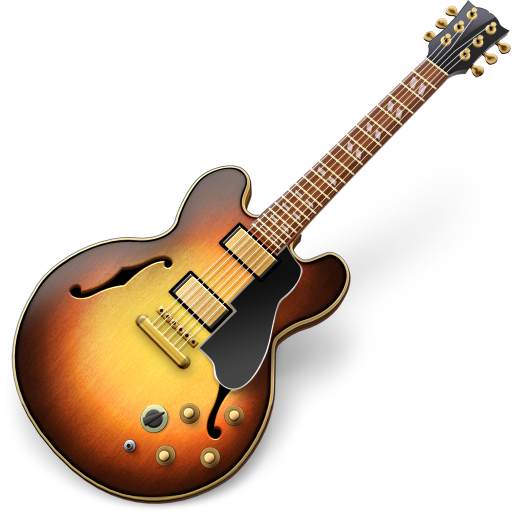
\includegraphics[width=2cm]{fig/garageband.png}
   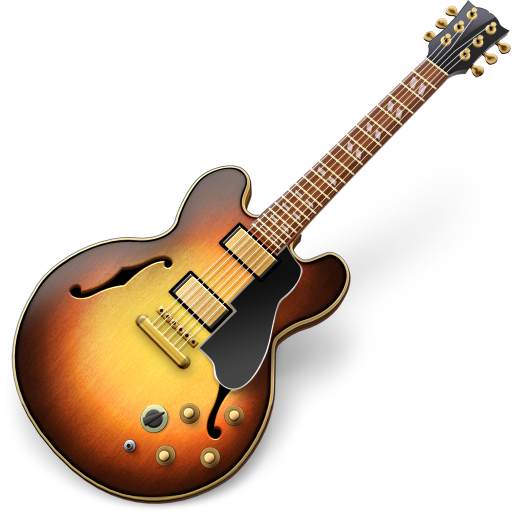
\includegraphics[width=1in]{fig/garageband.png}
   \label{fig:garagebaned}
\end{figure}

\section{Introduction}

In this activity we will cover the basics of music production using the popular digital audio workstation (DAW) GarageBand for the iPad. You will learn how to record, control, manipulate and remix the layers of a music session for the song ``Fast Enough'', by the band Infernal Devices. In the first part of the activity we will record some audio as a group that you can insert into your own remix. Then we'll get you familiar with how to work with audio and effects in Garageband. The point is to explore and be as creative as you like. Have fun!

\section{Getting Started}
To open GarageBand, locate the GarageBand icon on the iPad shown in the figure below. 
\begin{figure}[h]
   \centering
   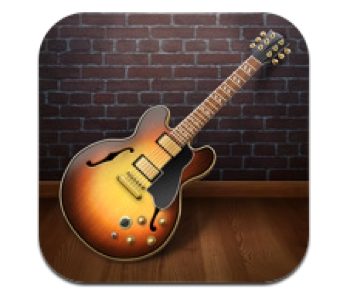
\includegraphics[width=0.8in]{fig/icon.jpg}
\end{figure}
You can swipe left or right to navigate to another screen if you don't see it. Once it opens, tap My Songs in the top left corner and you will see the songs currently on your iPad. Your screen should look like Figure \ref{fig:copy}. 
\begin{figure}[h]
   \centering
   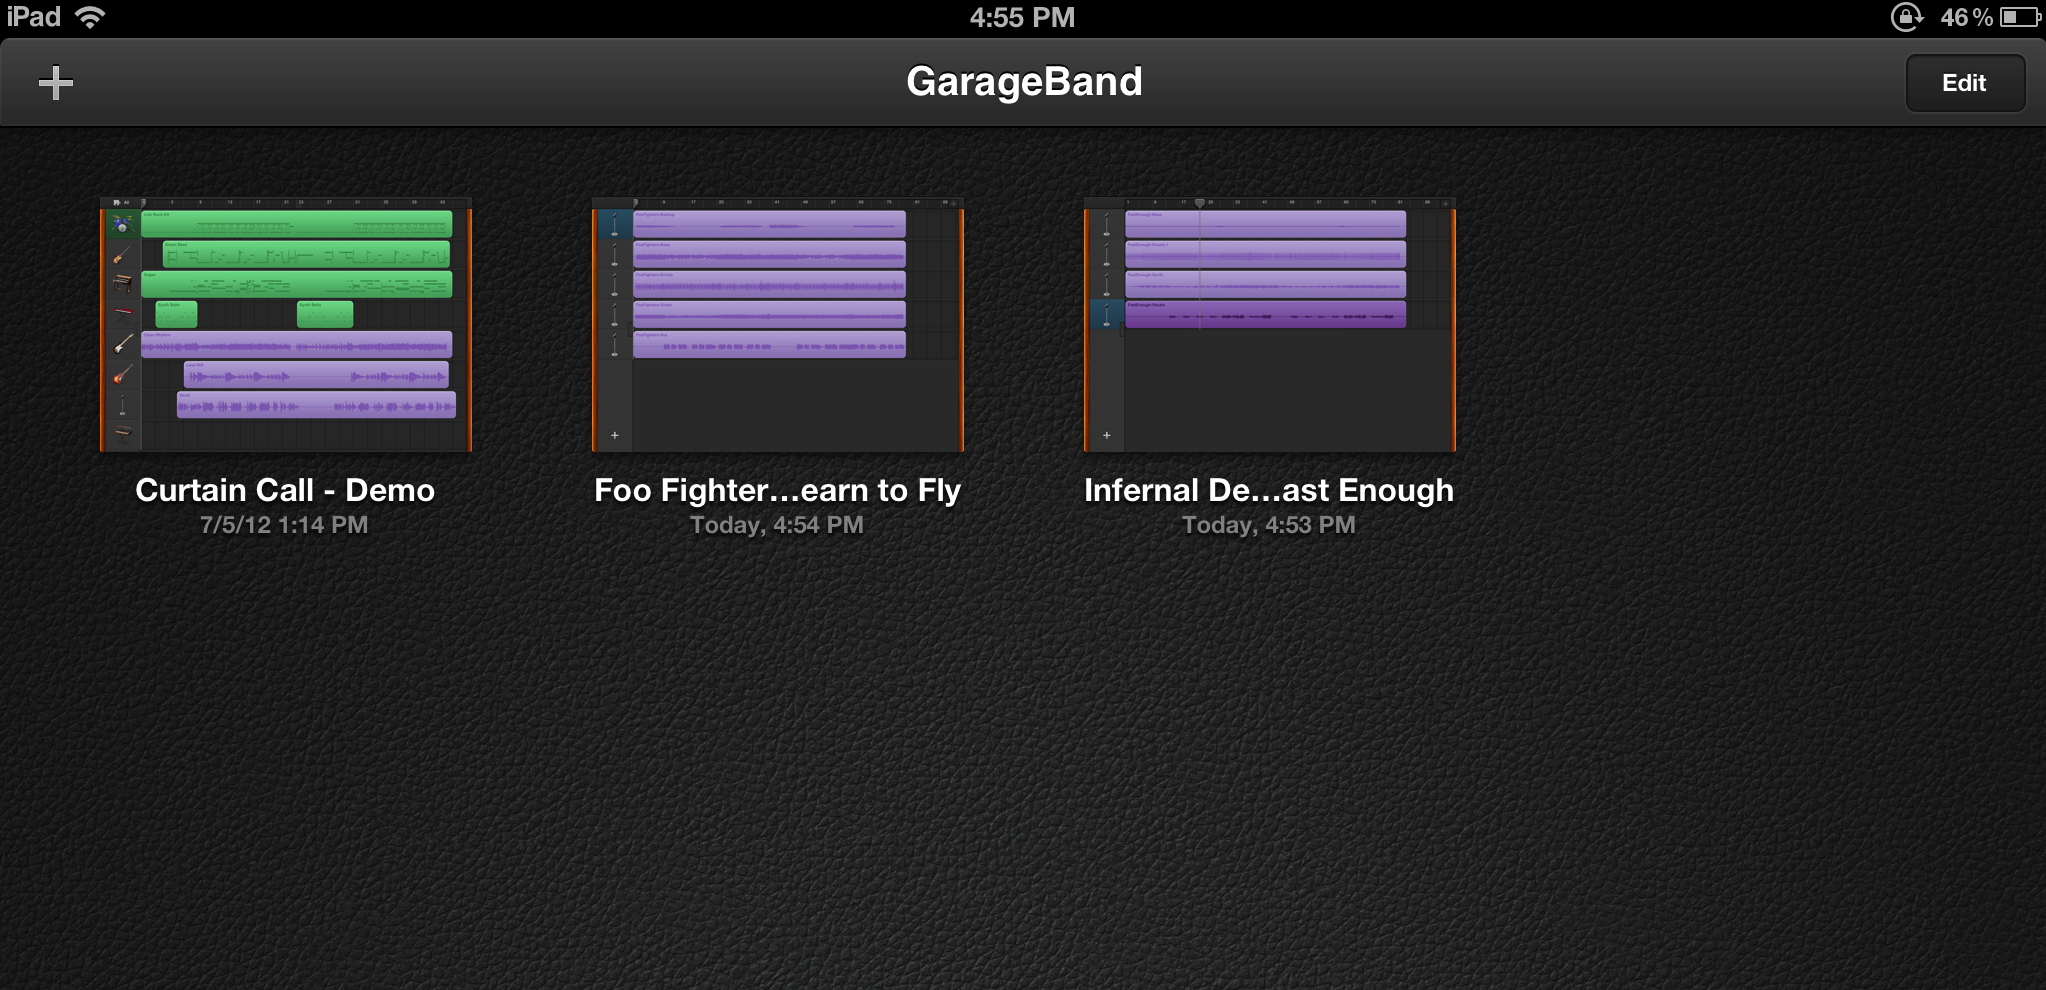
\includegraphics[width=4in]{fig/main_screen.png}
   \caption{Your Garageband song library. \label{fig:copy}}
\end{figure}
There are two songs, one song is an electronic song from Brooklyn based \emph{Infernal Devices} called Fast Enough. The other song is Learn to Fly by the \emph{Foo Fighters}. Tap the Fast Enough track for the tutorial, afterwards you can choose whichever song you want to remix.

% BASIC EDITING
\section{Basic Editing}\label{sec:basic_editing}
First we're going to learn how to cut up a track, move it around and loop sections.
\subsection{Region Editing}
\begin{figure}[h]
   \centering
   \includegraphics[width=4in]{fig/main.png}  
   \caption{The main project editing window.\label{fig:main}}
\end{figure}

Now you should be looking at the main project screen in Figure \ref{fig:main}. The numbers indicate the following controls:
\begin{enumerate}
   \item Playback controls
   \item Volume
   \item Editing/menus
   \item Track controls
   \item Add track
\end{enumerate}
\pagebreak
You can Pinch Close and Pinch Open to zoom in and out, respectively. Try it now. Now that you can zoom, let's start cutting up a track. Single tap the \emph{Drums} audio region to select it, then single tap again to bring up the editing options. 
\begin{figure}[h!]
   \centering
   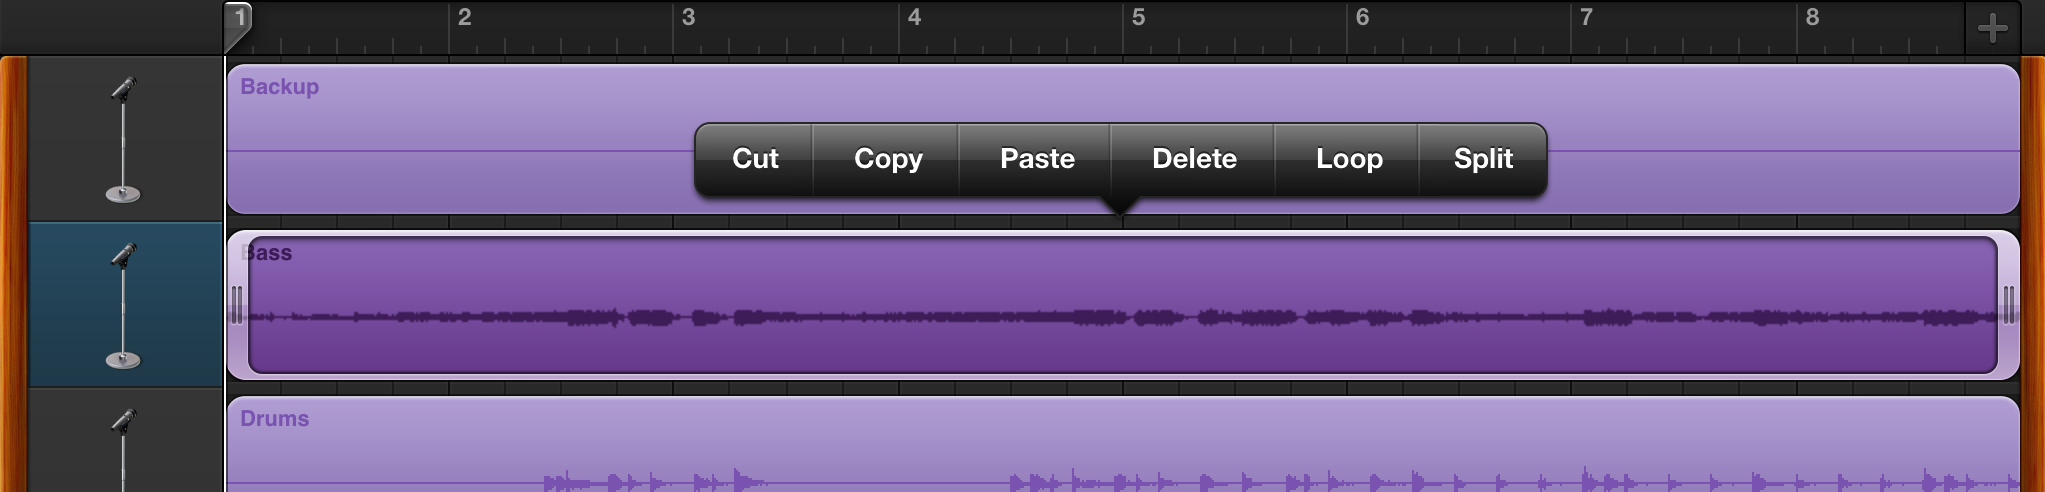
\includegraphics[width=5in]{fig/step1.png}  
   \caption*{The edit menu.\label{fig:edit}}
\end{figure}

Let's select Split to separate our region. Make sure you are zoomed in enough to see individual drum hits. Hold your finger on the scissor icon and drag it left or right to where you want to make the cut and then drag down. When you release your finger, you should have two separate regions.
\begin{figure}[h!]
   \centering
   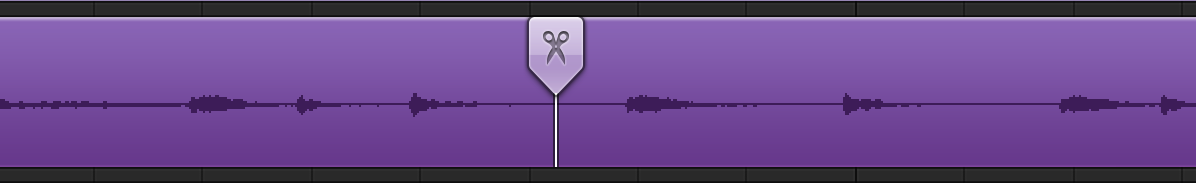
\includegraphics[width=4in]{fig/step2.png}
   \caption*{Splitting regions. \label{fig:slice}}
\end{figure}
Do the same thing on the other side of your drum hit. Now that you have your region sliced up, let's try looping it. 
\begin{figure}[h!]
   \centering
   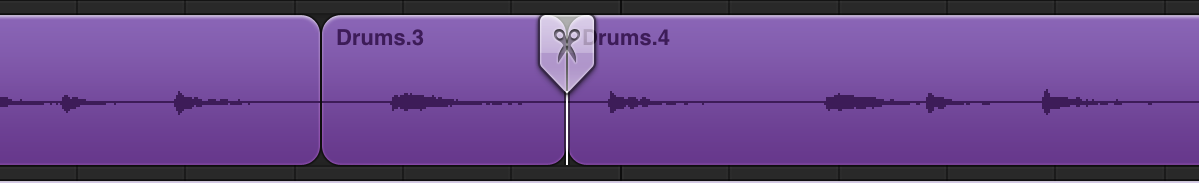
\includegraphics[width=4in]{fig/step3.png}
   \caption*{Splitting regions. \label{fig:slice}}
\end{figure}

Single tap the small region and it will be highlighted. You can drag the edges of the region to resize it as well as tap and drag the region to move it in the timeline. Clean up the edges and shorten the region tight to the waveform so that we can loop our clip.
\begin{figure}[h]
   \centering
   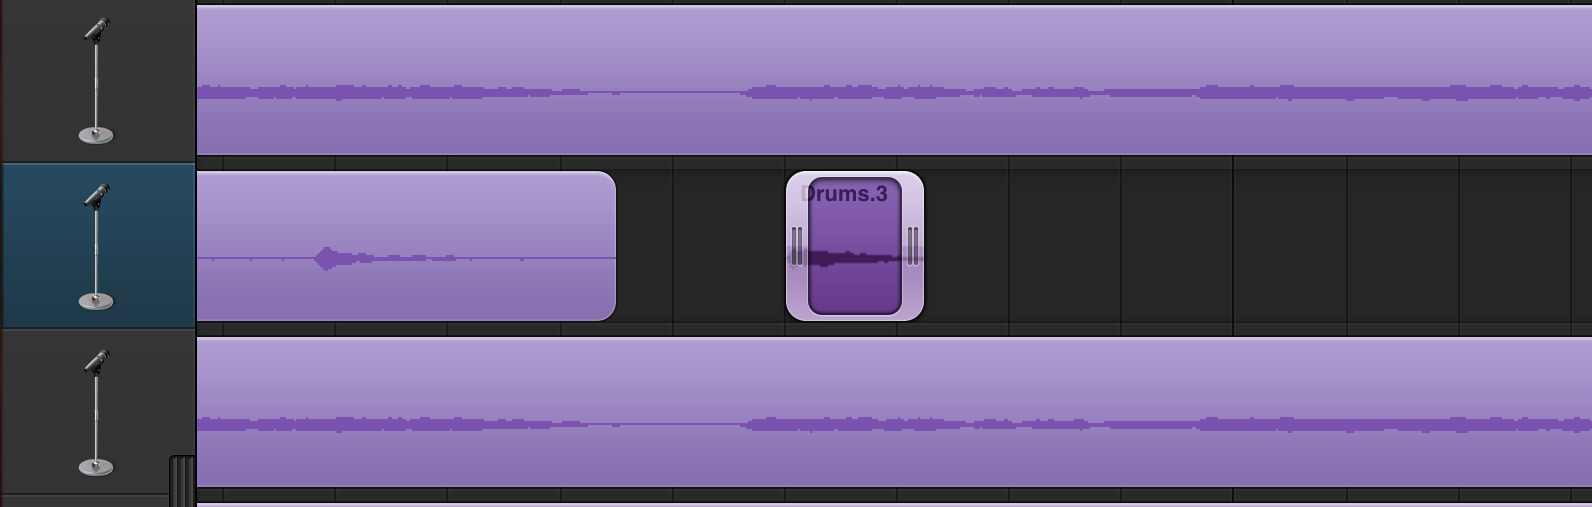
\includegraphics[width=5in]{fig/step4.png}
   \caption*{Shortened clip ready for looping.}
\end{figure}

Next single tap the region and select loop. Drag the loop icon to the right of the region to resize the length of the loop you just created (you can just drag it into the next region, it will push it to the left). You can single tap the region and then select trim to edit the size of the region that is looped. 

Let's solo our track so that we can listen to the loop by itself. Open the Track Controls (see the figure at the beginning of Section \ref{sec:basic_editing} if you don't recall how to do this). Now tap the headphone button, this will solo the track. Tapping the button to the left will mute the selected track. The slider to the right allows you to change the volume of an individual track. 
\begin{figure}[h]
   \centering
   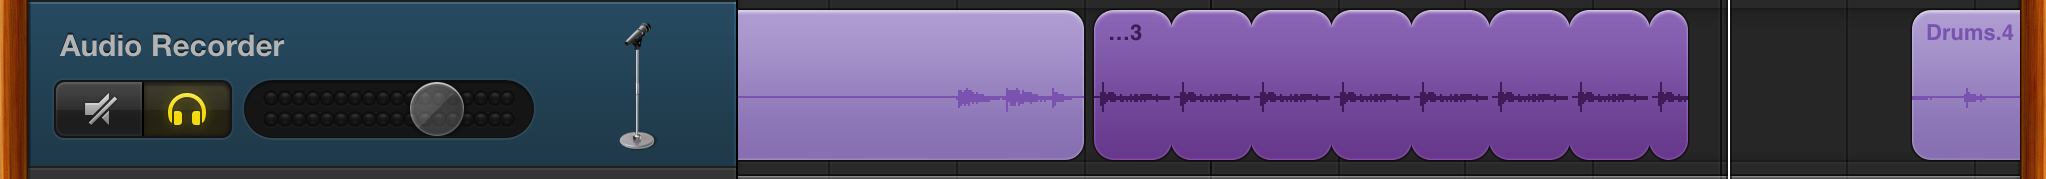
\includegraphics[width=6in]{fig/step5.png}  
   \caption*{Soloing a looped clip.}
\end{figure}

\subsection{More advanced editing}
Now that you have the basics of how to move things around, solo, mute and loop regions, let's get into some more advanced options. First let's add some effects. Tap the track that you want to add an effect to and then tap the mixer icon on the top left of the screen to open up the track edit window.
\begin{figure}[h]
   \centering
   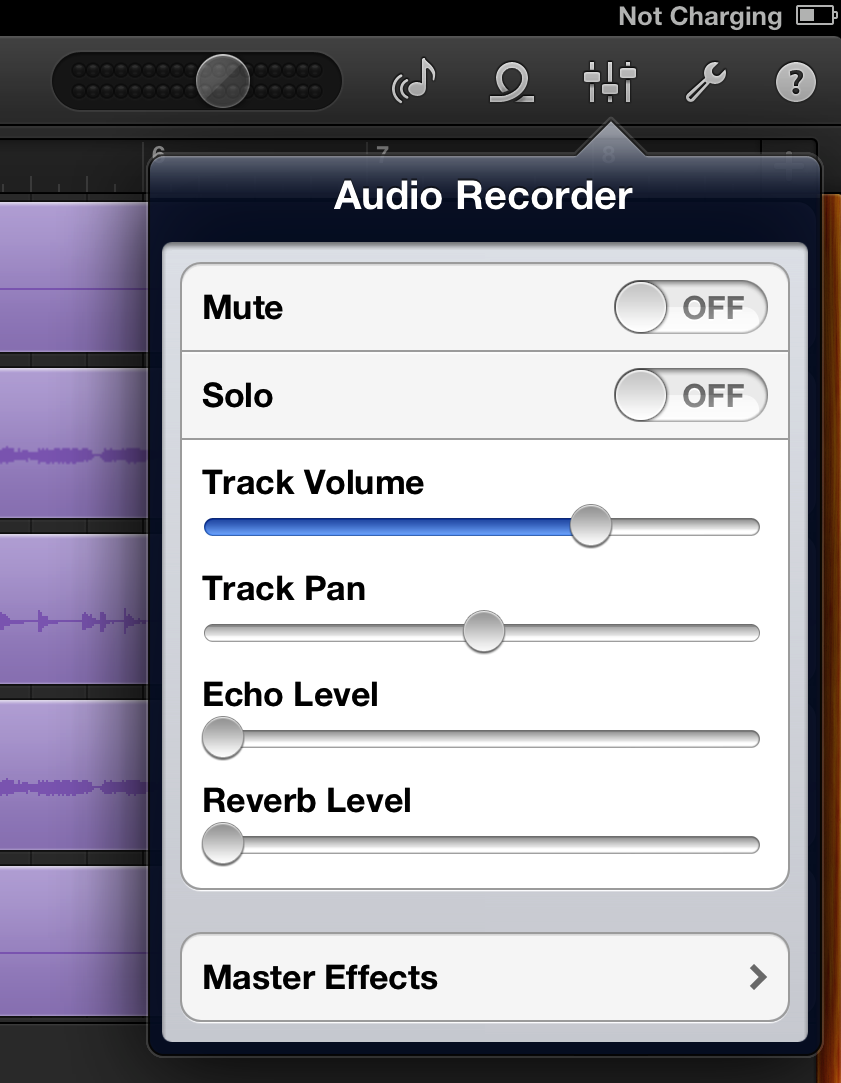
\includegraphics[width=3in]{fig/step6.png}
   \caption*{The track menu.}
\end{figure}

Now you can add echo (delay) and reverb to your track. Try adding some now and play around with each one individually as well as together. The Master Effects option let's you change the type of delay or reverb that is applied to the track but you can only have one delay or reverb type per session. You can also change the track panning using the slider in the track edit menu. If you're using headphones, it should be easy to hear the effect of moving the slider left or right.
\section{New Instruments}

GarageBand on the iPad allows you to add software instruments as well as audio tracks to your session.

\subsection{Adding Audio Tracks}
Let's add a loop to our song. We're going to add a tambourine to the chorus starting at bar 30. Open up the loop browser as shown in the screenshot below. Tap the instrument bar and then select Tambourine at the bottom left. Tap and drag ``Tambourine 01'' onto a new track and have it go from measure 30 to measure 46 (the chorus). Take the volume of the Tambourine track down a little bit so it sits better in the mix.
\begin{figure}[h]
   \centering
   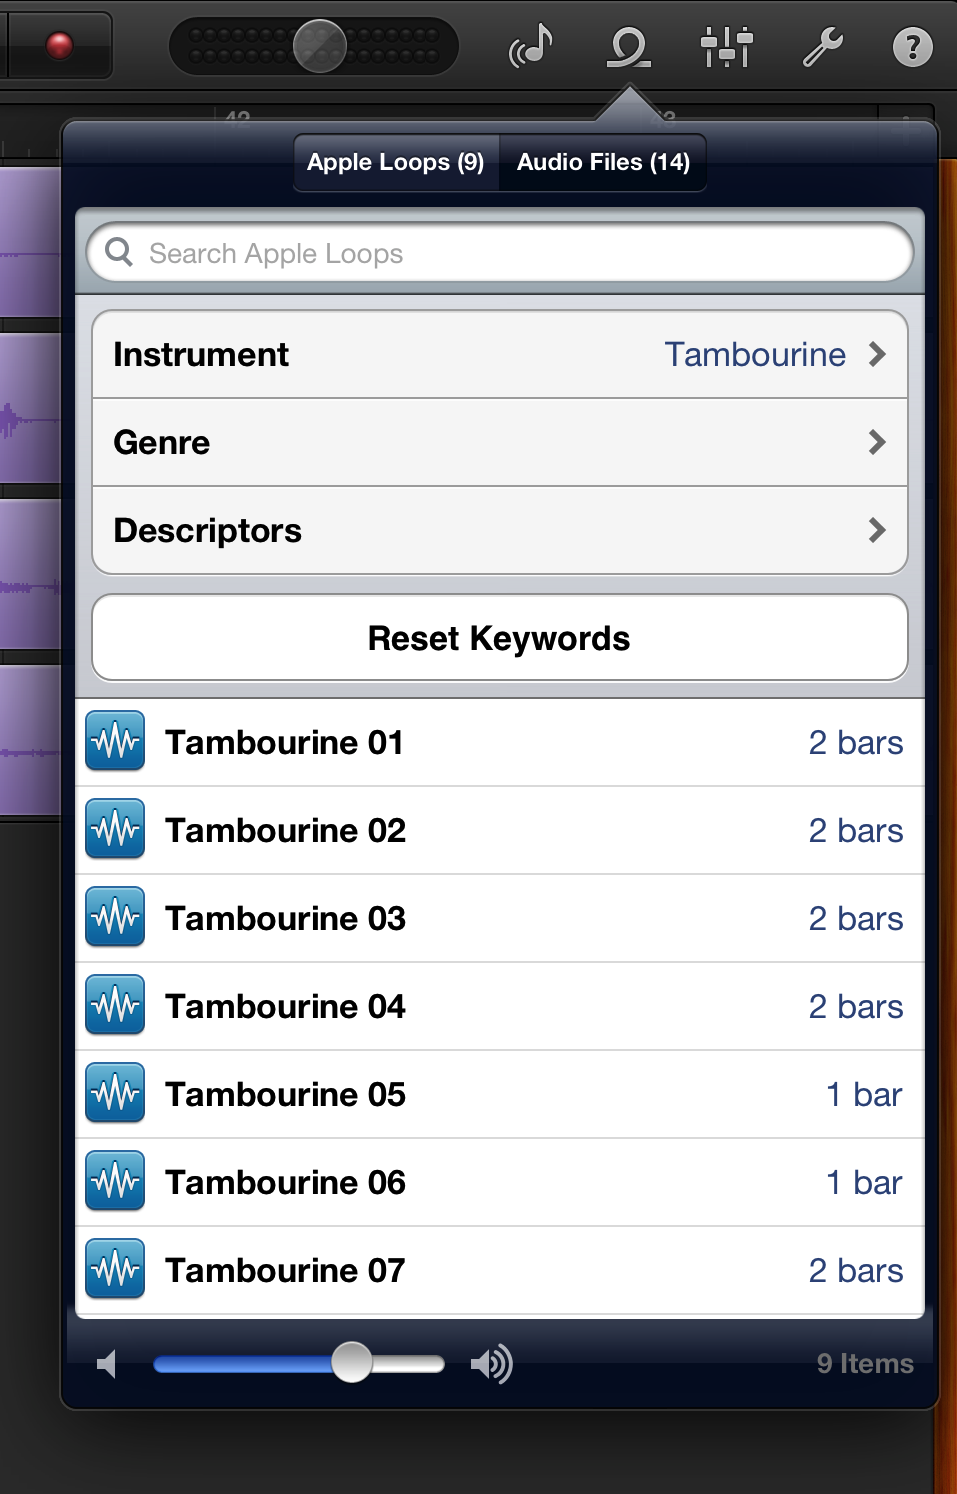
\includegraphics[width=2in]{fig/audio.png}  
   \caption*{Selecting a tambourine loop.}
\end{figure}

\subsection{Adding Software Instruments}
To add an instrument, tap on the Instruments button at the top left of the screen. Swipe left or right to browse through the instruments that are available. Let's add a synthesizer patch, so swipe until you get to Keyboard and then tap to select it. 
\begin{figure}[h]
   \centering
   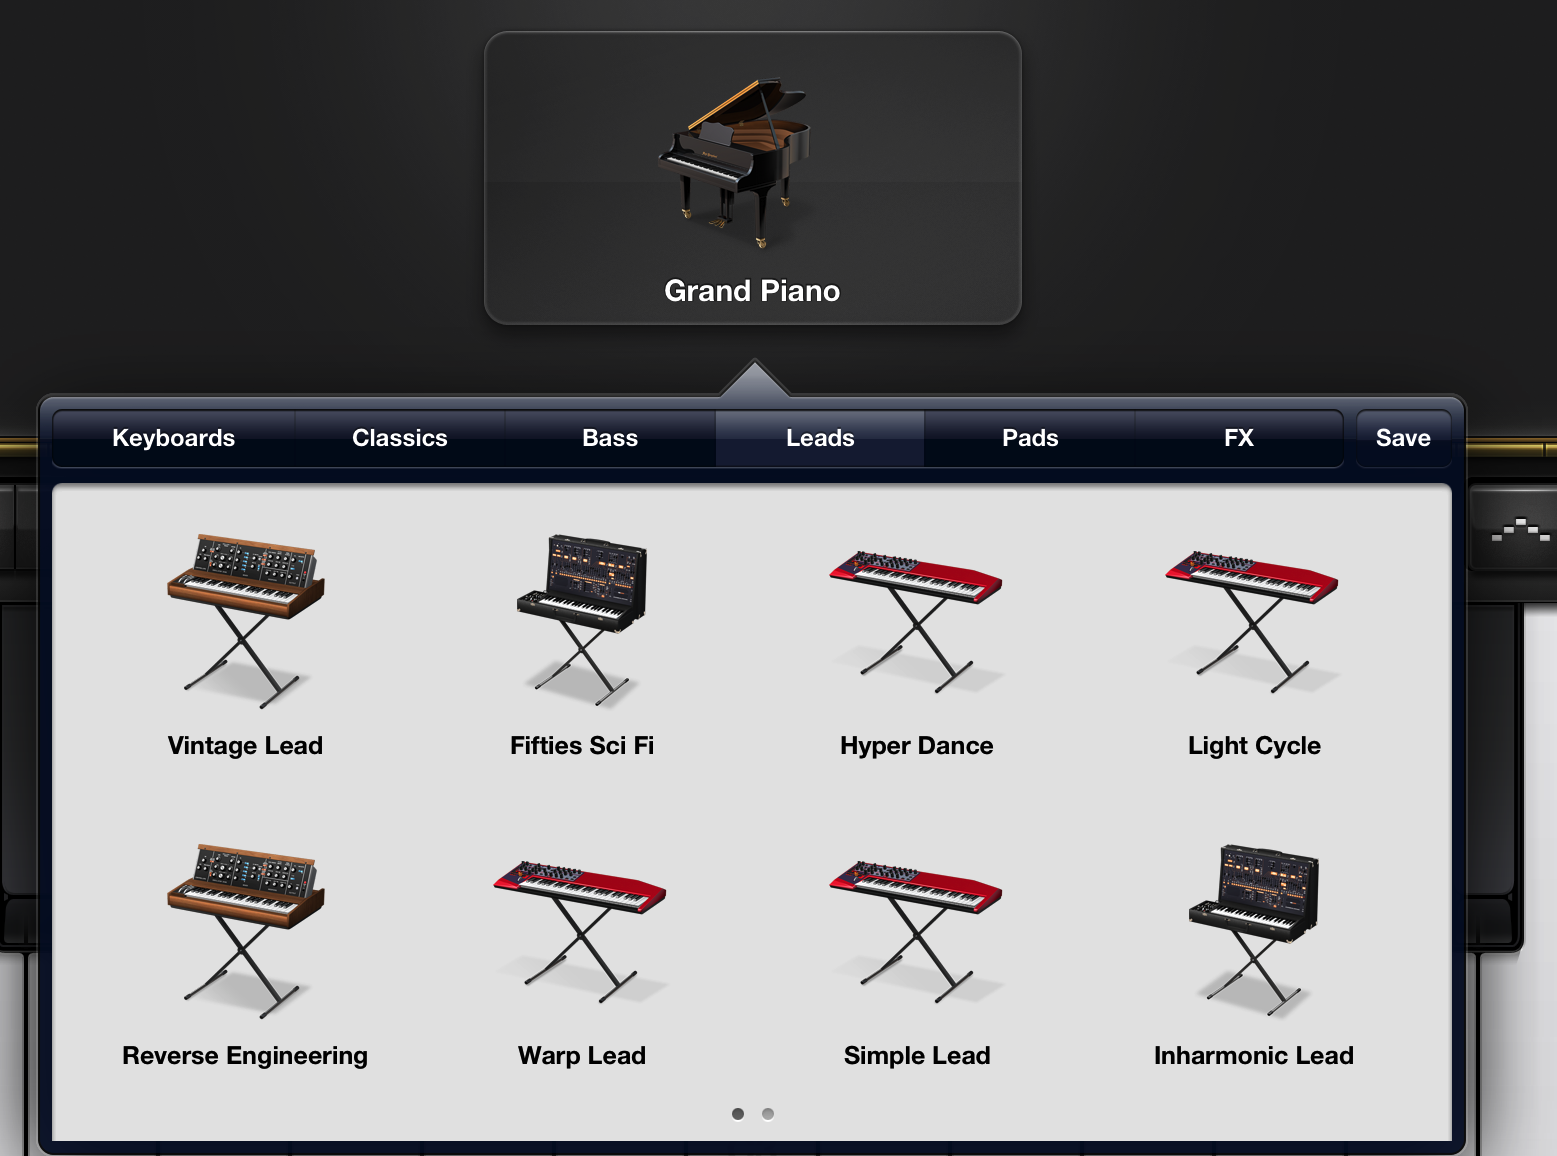
\includegraphics[width=4in]{fig/inst1.png}
   \caption*{Loading the Warp Lead synth patch.}
\end{figure}
The Grand Piano instrument comes up, but that's not what we want so tap the Grand Piano picture. Tap the Leads tab and then select Warp Lead from the menu that appears.
\begin{figure}[b!]
   \centering
   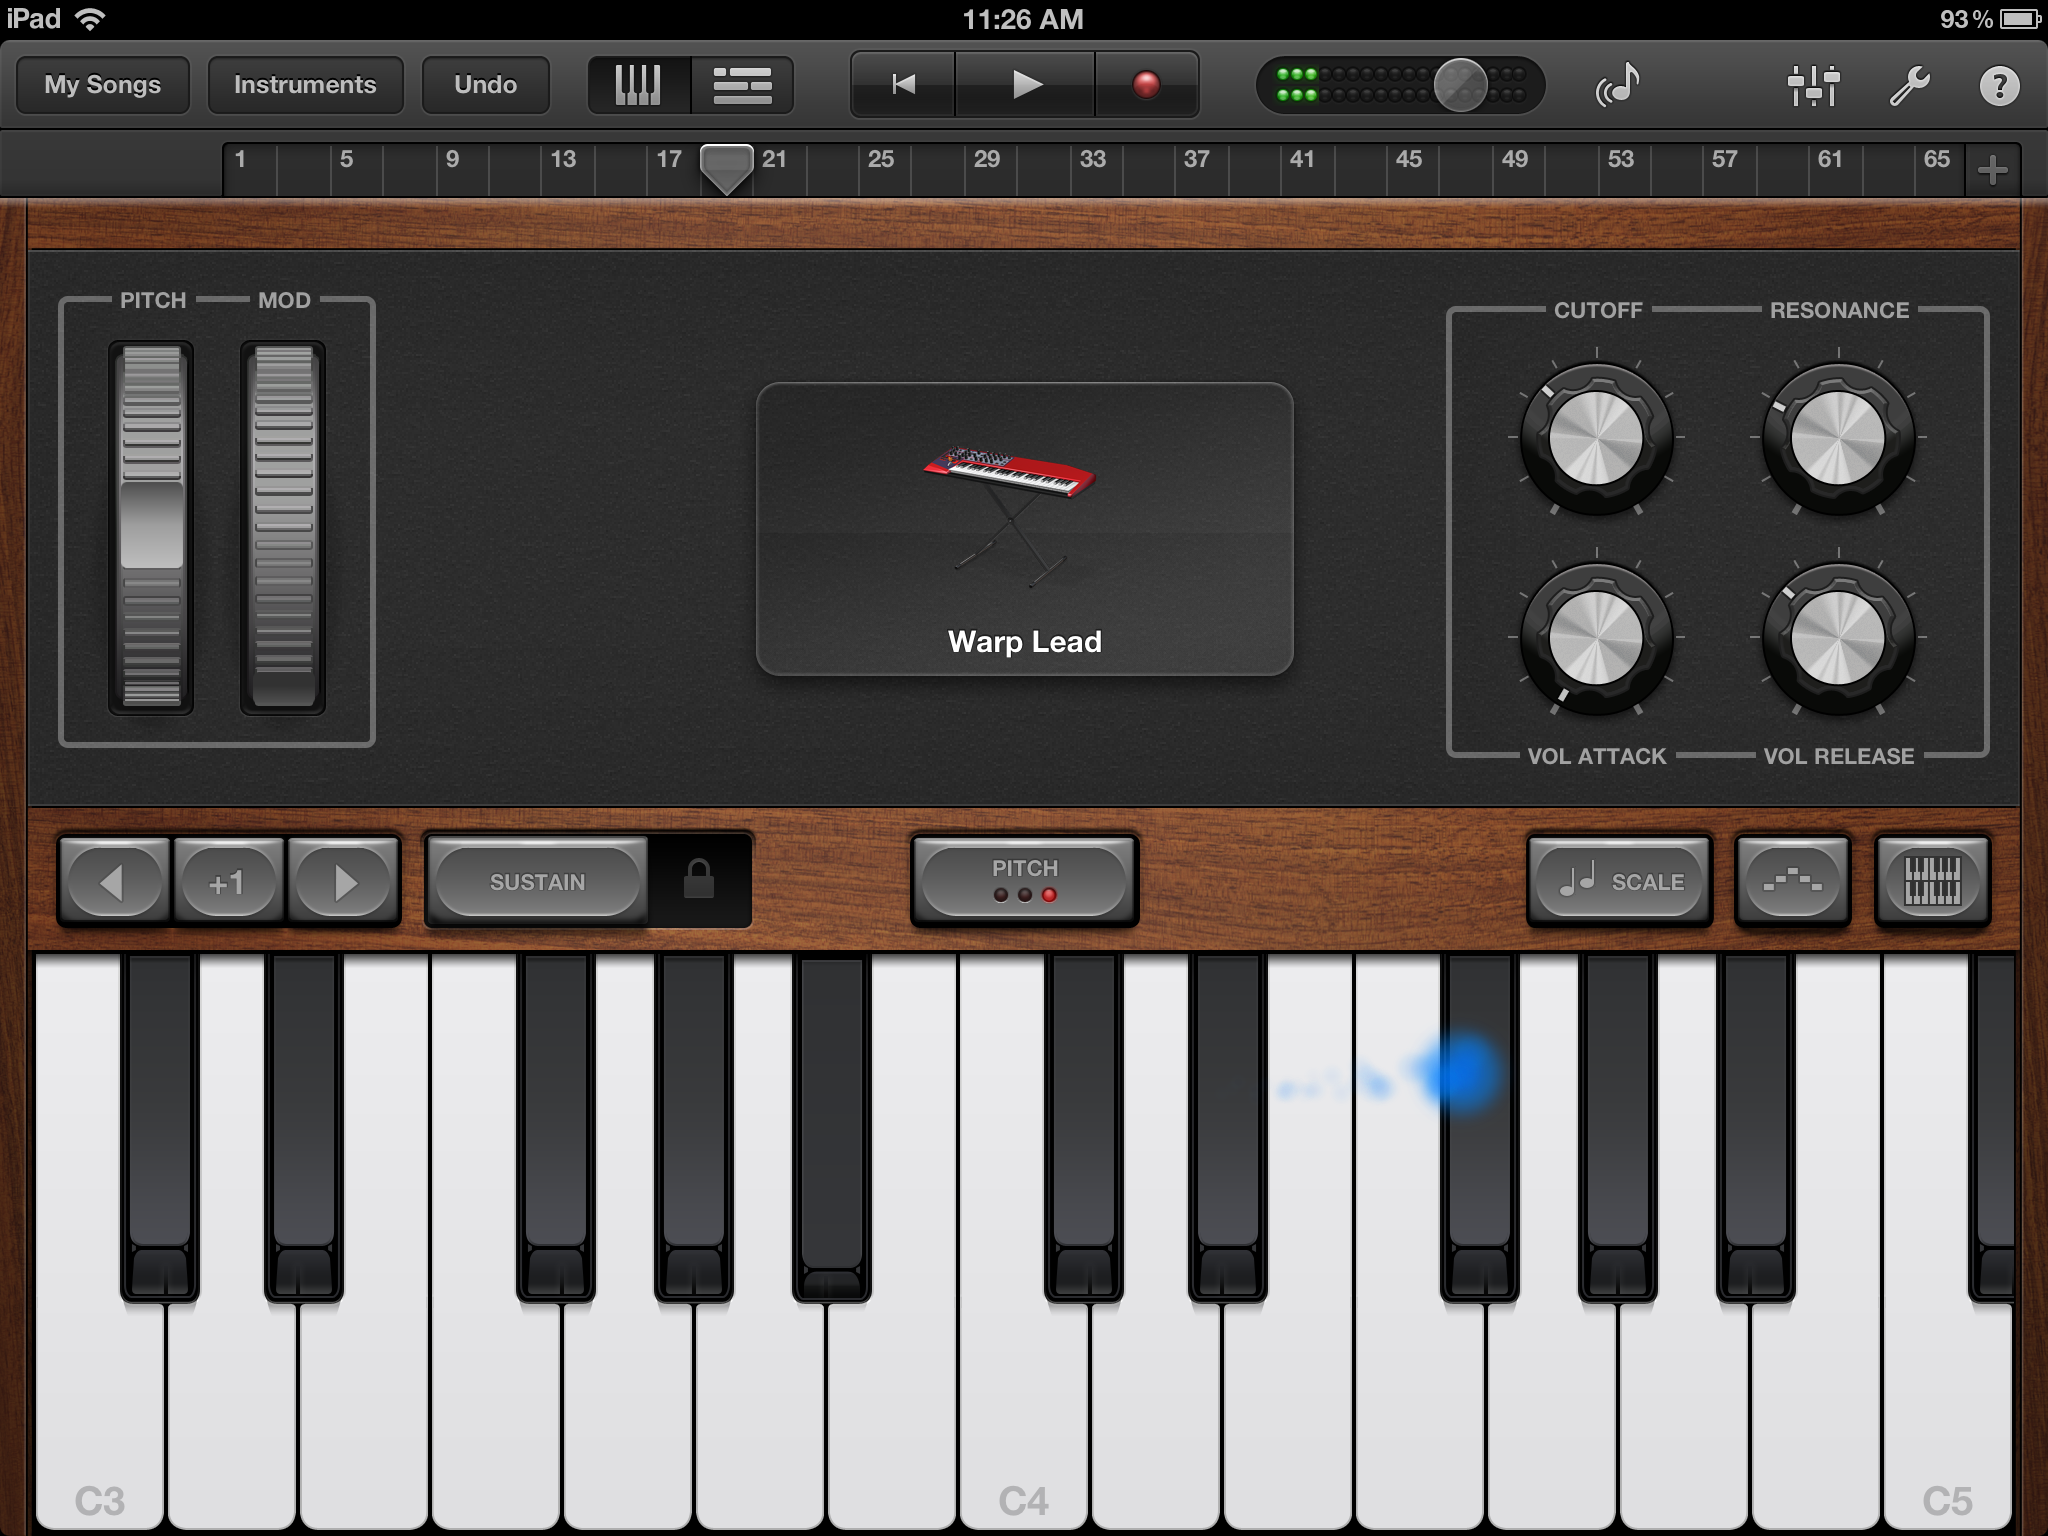
\includegraphics[width=3in]{fig/inst2.png}
   \caption*{The Warp Lead synth patch.}
\end{figure}
Now you have a parameterized synthesizer to play around with. The keyboard does what you would expect it to. Play around with the pitch and modulation wheels on the left as well as the filter parameters (cutoff/resonance/attack volume/release volume) on the right. Once you find a sound that you like, you can hit record (red dot) at the top of the screen and add the layer to your remix. To get back to the arrange window, hit the button to the left of the playback controls that looks like a set of audio regions.

\pagebreak

\section{Finishing Up}
If you want to save your song, you can export it to iTunes. Tap `My Songs' to get back to the main menu. Hit the edit button at the top left of the screen and then single tap your song. Tap the icon on the top left that has the arrow. Select `Share Song Via Mail' and follow the instructions.
\begin{figure}[h]
   \centering
   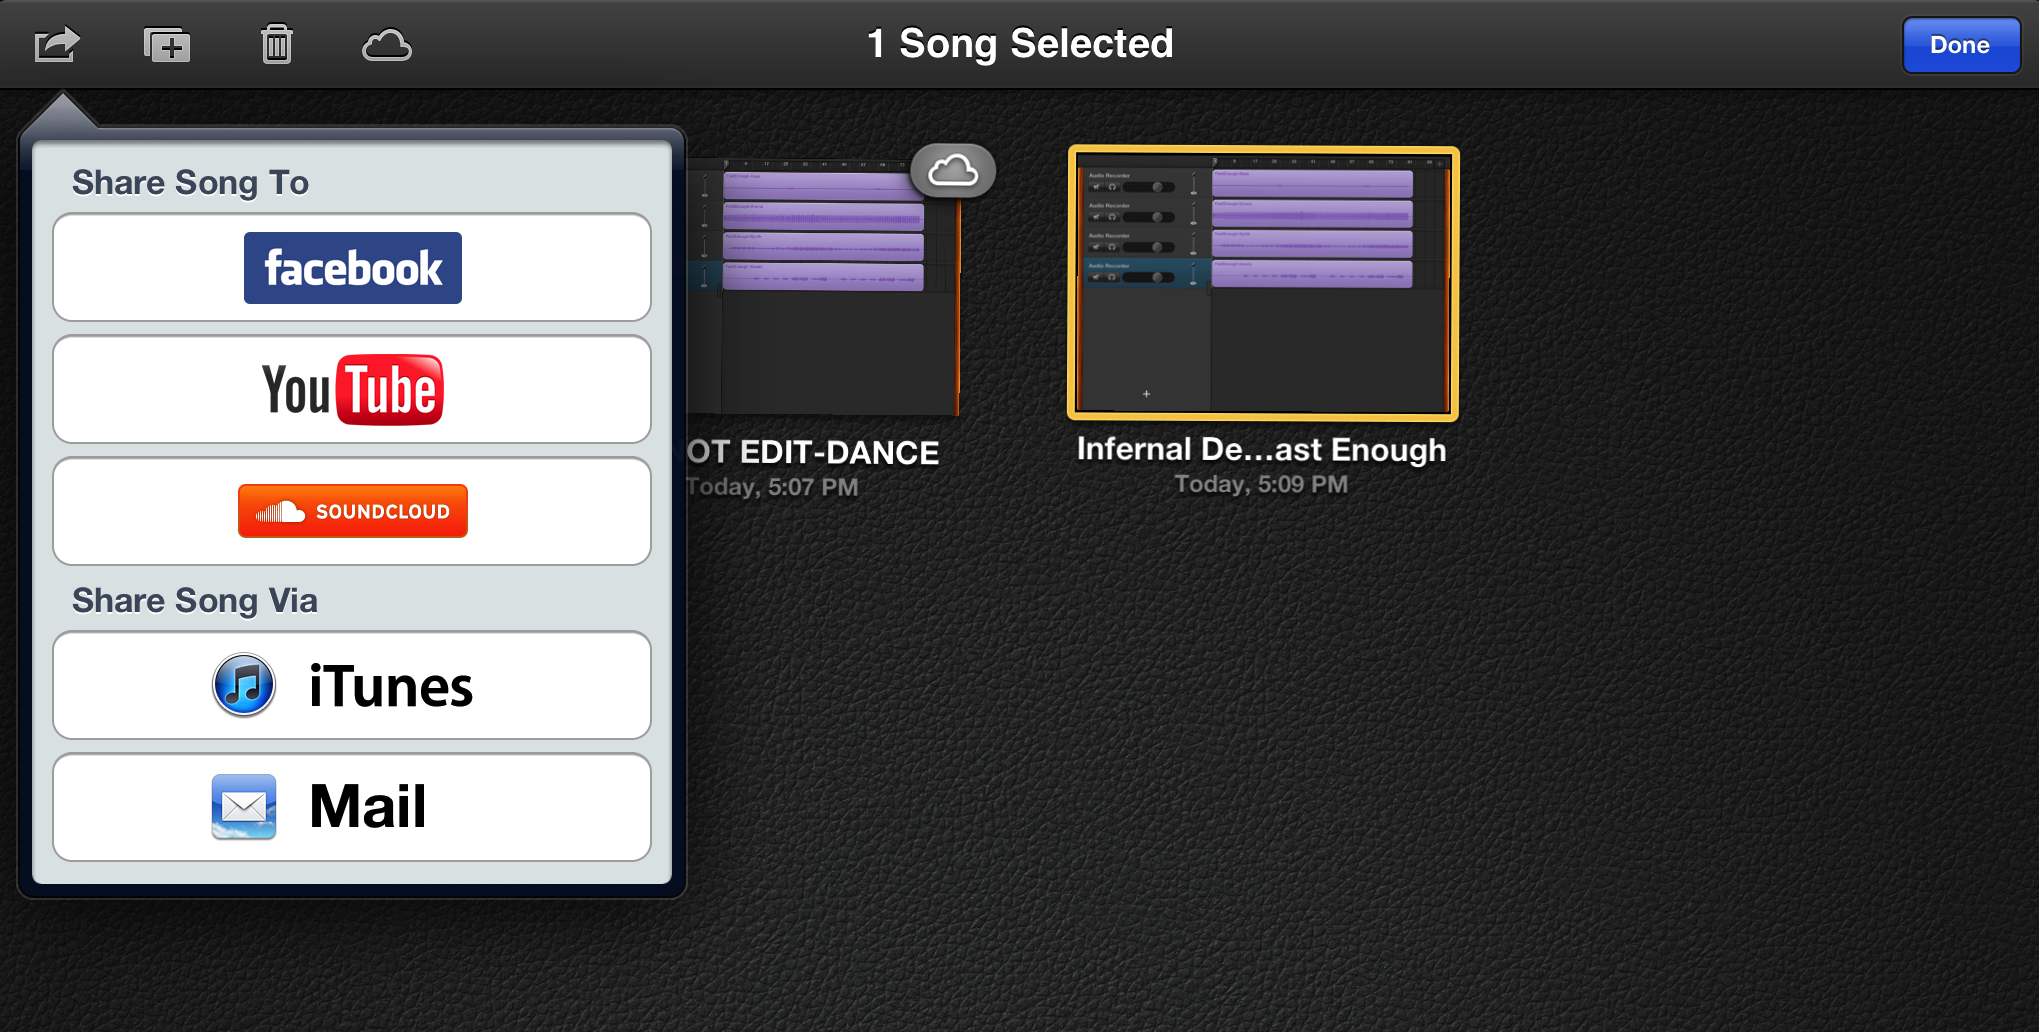
\includegraphics[width=5in]{fig/share.png}
   \caption*{Exporting your song.}
\end{figure}

\noindent Now feel free to continue editing your song and exploring the possibilities of GarageBand. There are several songs available for you to remix. Have Fun!
\end{document}